
As shown in \cref{fig:diagram_Connectivity-Activity}, our idea for connection inference rests on the causal `presynaptic spike' → `postsynaptic voltage bump' link. I.e. we want to know for which neuron pairs a spike in one is reliably followed by such a bump in the other. The problem is that these bumps (the postsynaptic potentials or PSPs) are minute, and are easily drowned out by (1) other PSPs, (2) postsynaptic spikes, and (3) voltage imaging noise.

So, as is often done in neuroscience, we take the \emph{average} over many instantiations, so as to hopefully find a signal in the noise. Specifically, we take spike-triggered averages, or \textbf{STA}s, of neurons' voltage traces. If there is a connection from neuron `M' to neuron `N', then an STA of neuron N's voltage imaging signal, based on neuron M's spikes, would hopefully show the PSP.

To use this idea for an actual connection test, we look specifically at the height of an STA, and compare it to a distribution of STA heights that we'd expect were the two neurons not connected. This is illustrated in \cref{fig:STA-height-suffle}.


\begin{figure}
    \vspace*{2em}
    \hspace*{-1em}
    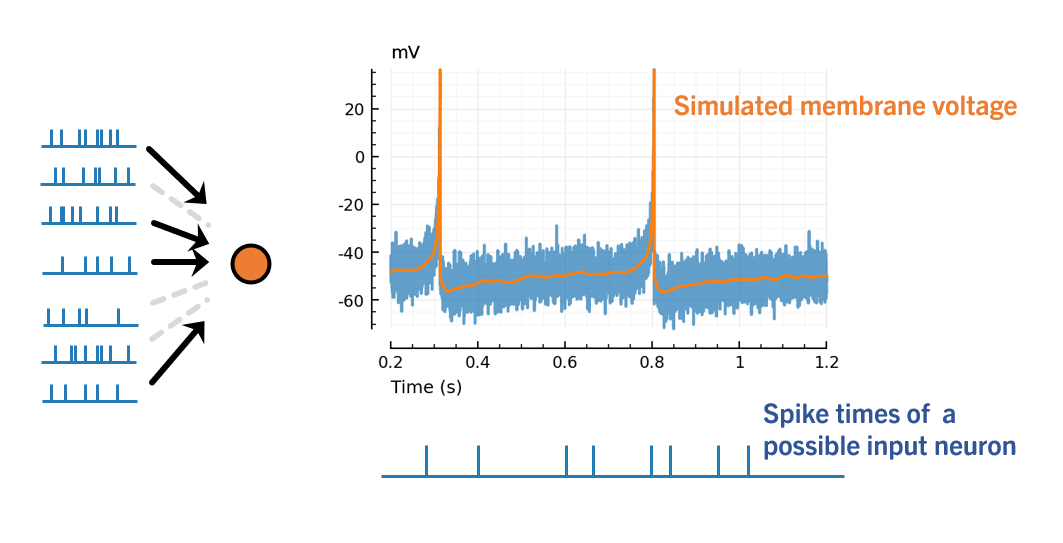
\includegraphics[w=1.2]{diagram_Nto1.png}
    \vspace*{-1.4em}
    \captionn
        {The `N-to-1' problem}
        {\Left: A neuron $N$ (orange circle), and the spike trains of other neurons in the network (blue). Some of these other neurons impinge directly on $N$ (black arrows), while others are not (directly) connected (dashed gray lines). Given only neuron $N$'s voltage signal and the other neurons' spiketrains, we want to detect the direct inputs, while rejecting the not-directly-connected spiketrains.\newline
        \Right: The simulated membrane voltage of the impinged-upon neuron (orange), and the same signal with Gaussian noise added, to simulate a voltage imaging signal (blue). Underneath the plot, one of the possible input spiketrains, time-aligned to the voltage signal.
        This alignment is used later to extract spike-triggered windows from the voltage signal.}
    \label{fig:diagram_Nto1}
\end{figure}

\begin{figure}
    \hspace{-5em}
    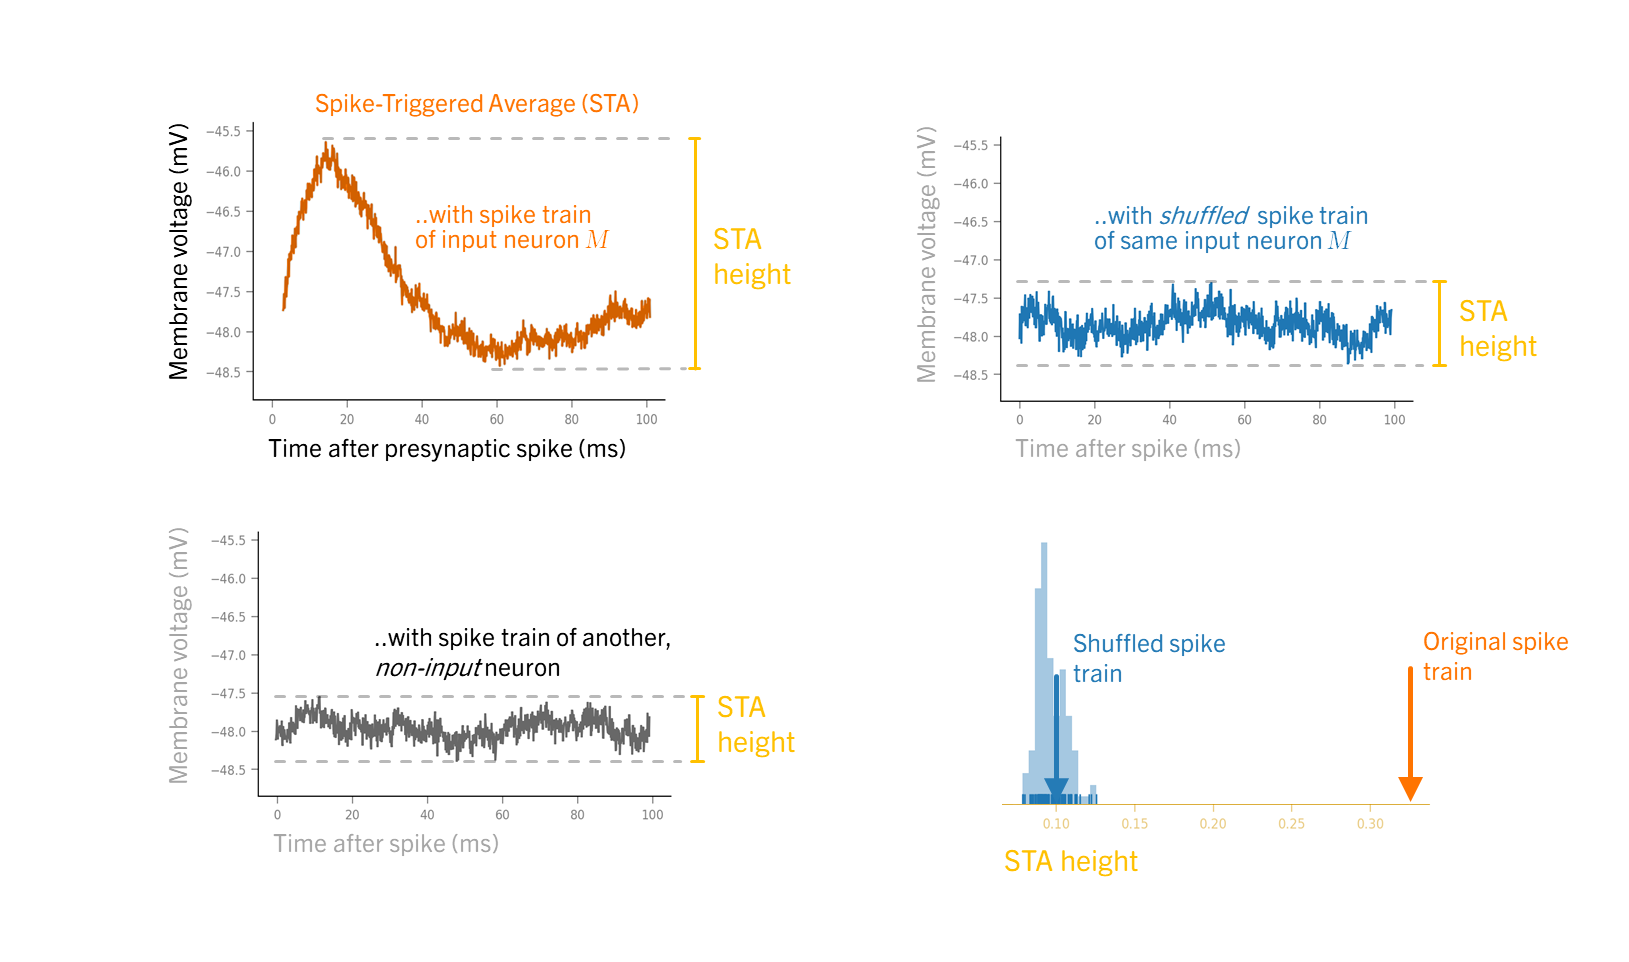
\includegraphics[w=1.7]{diagram_STA_test.png}
    \captionn
        {A simple connection test: STA height with shuffle control}
        {The spikes of a possible input neuron are aligned to the voltage trace of the neuron of interest $N$, as in \cref{fig:diagram_Nto1}. For every such spike, a 100-ms long window is cut out of the voltage of $N$. The average of all these windows is called the spike-triggered average (STA).\newline
        \Left: Two example STAs of neuron $N$'s membrane voltage: one for an actually connected input neuron, $M$ (top, orange); and one for a non-input neuron (below, gray).
        Given an STA signal $x$, we will use its height $h = \max(x) - \min(x)$ (also known as `peak-to-peak' or `ptp') to test whether two neurons are connected. \newline
        \Right: An STA of $N$'s membrane voltage using a shuffled version of $M$'s spike times (which is made by randomly permuting the inter-spike-intervals of $M$). This `shuffled STA height' provides a control for the STA height connection test statistic: "what do we expect the STA height to be if there is \emph{no} connection $M$→$N$".
        By calculating different such shuffles, we obtain a null-distribution for the STA height test statistic. And by comparing the real STA height to this distribution, we can calculate a $p$-value. Here, the real STA is larger than all shuffle controls, of which there are 100. So $p < 0.01$, and at α = 0.05, we conclude there is indeed a connection $M$→$N$.}
    \label{fig:STA-height-suffle}
\end{figure}

\begin{figure}
    \hspace*{-3em}
    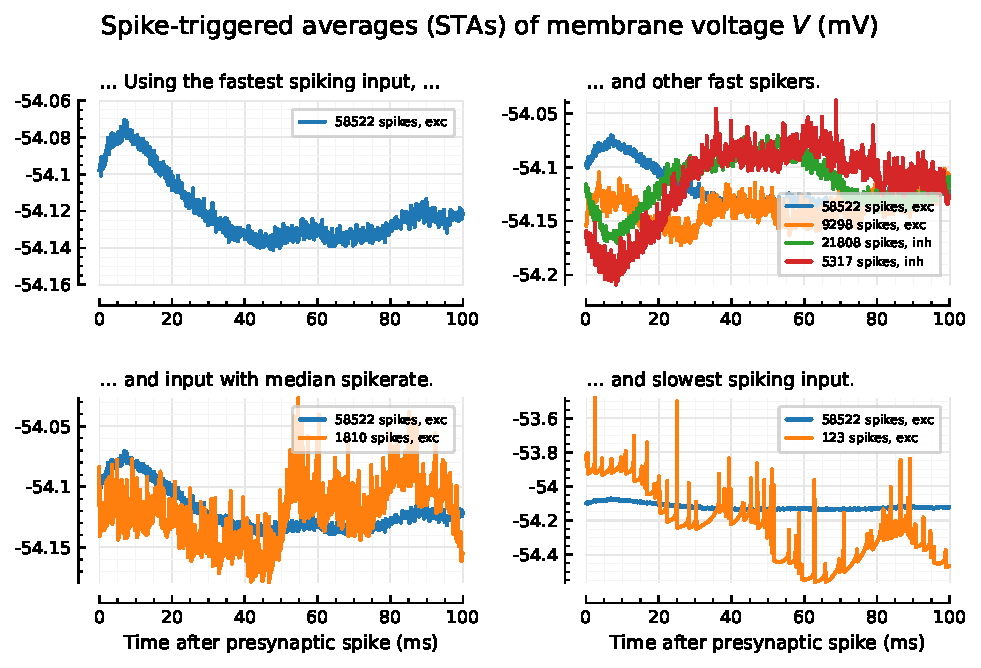
\includegraphics{example_STAs}
    \vspace*{1em}
    \captionn
        {Example STAs in the 10' simulation with 6500 inputs}
        {
        Note that every panel has a different y-axis (voltage) scale. The STA of the most active input is repeated in every panel (in faded blue), to allow a visual scale comparison nonetheless.\\
        The inset legends indicate with how many presynaptic spikes the STA was calculated, and whether the input was an excitatory or inhibitory one.\\
        The top right panel shows STAs of the 1\ts{st} and 100\ts{th} fastest spiking inputs, both within the excitatory inputs (\mpl{blue} shades), and within the inhibitory inputs (\mpl{orange} shades).\\
        Source: \nburl{2023-09-13__Clippin_and_Ceilin}.
        }
    \label{fig:example_STAs}
\end{figure}


\FloatBarrier
\section{Ceiling and clipping}
\label{sec:ceil-n-clip}



\begin{figure}
    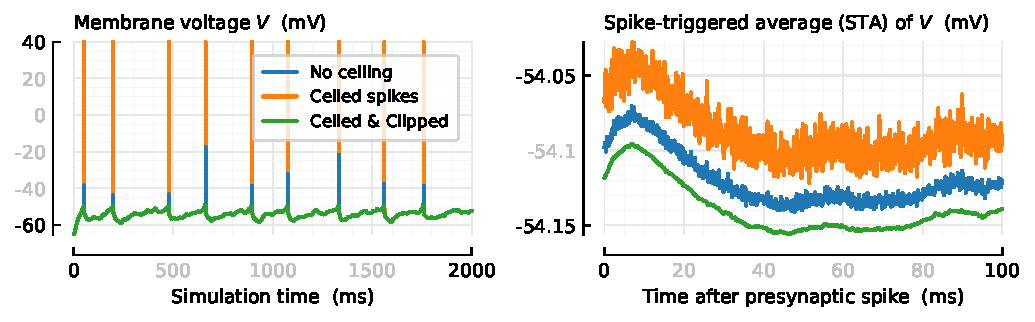
\includegraphics{ceil_n_clip__sigs_and_STAs}
    \captionn
        {}
        { }
    \label{fig:ceil_n_clip__sigs_and_STAs}
\end{figure}

\begin{figure}
    \begin{sidecaption}
        {}
        [fig:ceil_n_clip_AUCs]
        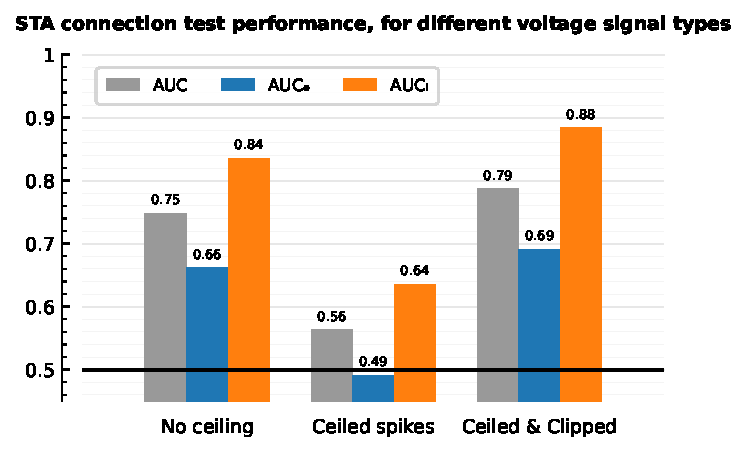
\includegraphics{ceil_n_clip_AUCs}
    \end{sidecaption}
\end{figure}


\FloatBarrier
\section{Performance quantification}

% \rule[0.5ex]{4.5in}{0.55pt}

\begin{figure}
    \includegraphics{perfmeasures_θ_TPR_ROC}
    \captionn
    { }
    {Source: \nburl{2023-09-13__Clippin_and_Ceilin}.}
    \label{fig:perfmeasures_θ_TPR_ROC}
\end{figure}

\begin{figure}
    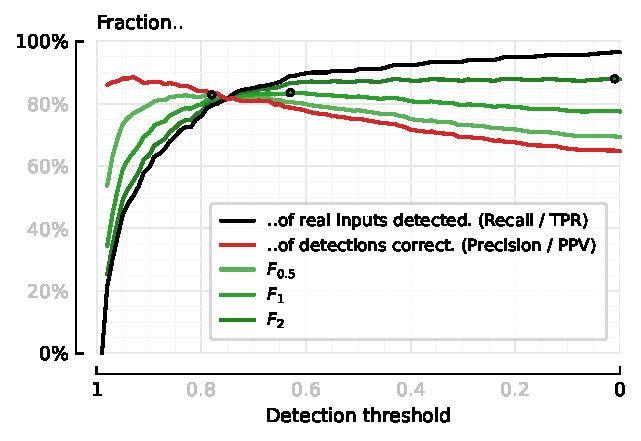
\includegraphics{perfmeasures_Fscores}
    \captionn
        {}
        {}
    \label{fig:perfmeasures_Fscores}
\end{figure}

\begin{figure}
    \includegraphics{PR_curves_iso_Fβ}
    \captionn
        { }
        {}
    \label{fig:PR_curves_iso_Fβ}
\end{figure}

\begin{figure}
    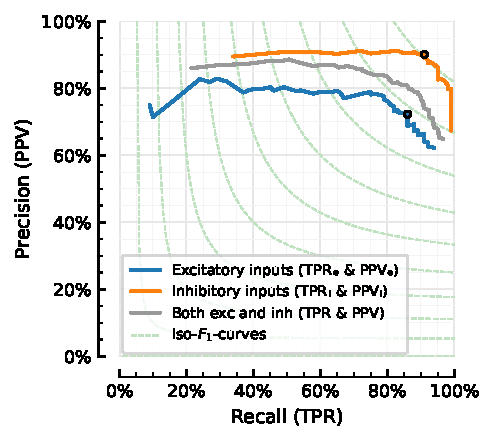
\includegraphics{perfmeasures_PR_curves_EI}
    \captionn
        {}
        {}
    \label{fig:perfmeasures_PR_curves_EI}
\end{figure}

\begin{figure}
    \begin{sidecaption}
        {\textbf{Excitatory and inhibitory inputs reach \maxF at different thresholds}.\\
        But for simplicity, whenever we use \maxF to evaluate a classifier, we will use only one threshold for both types of inputs, which will be a compromise between these two thresholds.}
        [fig:perfmeasures_threshold_PPVs_EI]
        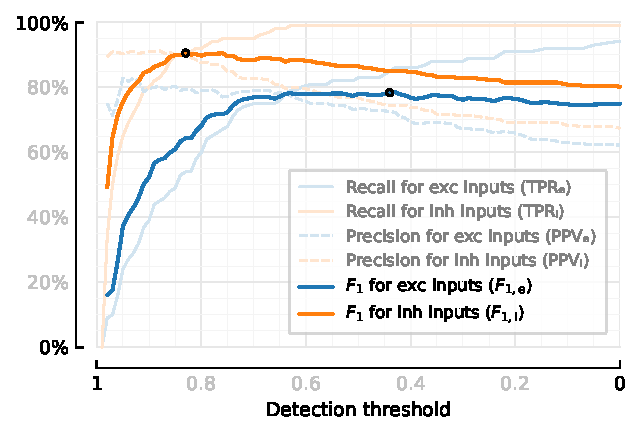
\includegraphics{perfmeasures_threshold_PPVs_EI}
    \end{sidecaption}
\end{figure}

\begin{figure}
    \begin{sidecaption}
        {\textbf{Randomly classifying connections yields a chance level AUC $< 0.5$}.\\
        300 random test results, and their performance as connection detector, quantified as area under their ROC curves. Solid black line is the mean, dashed line is the median.\\
        In every of the 300 simulations, every connection (100 exc, 100 inh, and 100 unconnecteds) was assigned a random `t-value' uniformly between $-1$ and $1$; and then the classification threshold was swept over these t-values.}
        [fig:AUC_chance_level]
        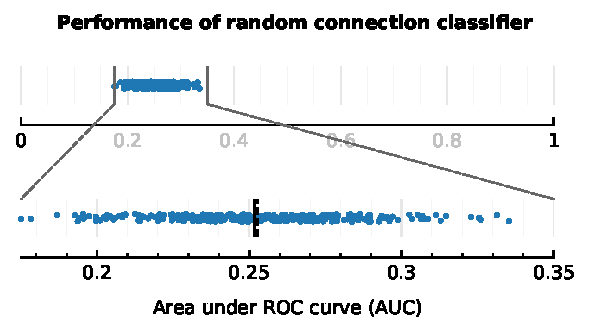
\includegraphics{AUC_chance_level}
    \end{sidecaption}
\end{figure}



\FloatBarrier
\section{Recording duration \& noise}

\begin{figure}
    \begin{sidecaption}
        {\textbf{Performance drops to chance level for noisier signals}.\\
        All simulations were 10 minutes long.
        Signal-to-noise (SNR) values on the x-axis are approximately (but not exactly) log-spaced. An SNR of `$\infty$' corresponds to no noise (i.e. the voltage signal straight out of the simulation, without any noise added).
        For every SNR value, five different simulations were run (gray dots), each with a different RNG seed for input firing rate and spiketrain generation. The mean performances of these five simulations are plotted with larger dots and are line-connected.
        Only the 100 highest-firing excitatory and inhibitory inputs were tested. An additional 100 unconnected spiketrains were generated and tested, with similar firing rates as those 200 high-firing real inputs.\\
        AUC chance level determined as in \cref{fig:AUC_chance_level}.\\
        Source: \nburl{2023-09-20__STA_conntest_for_diff_recording_quality_n_durations}.}
        [fig:STA_perf_diff_snr]
        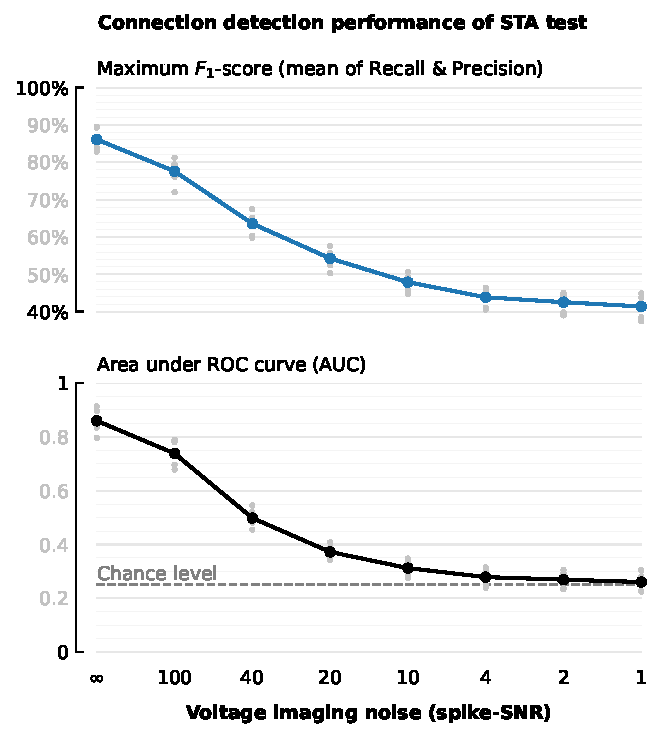
\includegraphics{STA_perf_diff_snr}
    \end{sidecaption}
\end{figure}

\begin{figure}
    \begin{sidecaption}
        {\textbf{Longer recordings allow more accurate connection inference}.\\
        All simulations had a voltage imaging noise level (spike-SNR) of 40.\\
        The simulation (`recording') durations are on a logarithmic axis. (The first two data points are at 10 and 30 seconds; the last one is at 1 hour). \\
        For more, see \cref{fig:STA_perf_diff_snr}'s caption.}
        [fig:STA_perf_diff_rec_duration]
        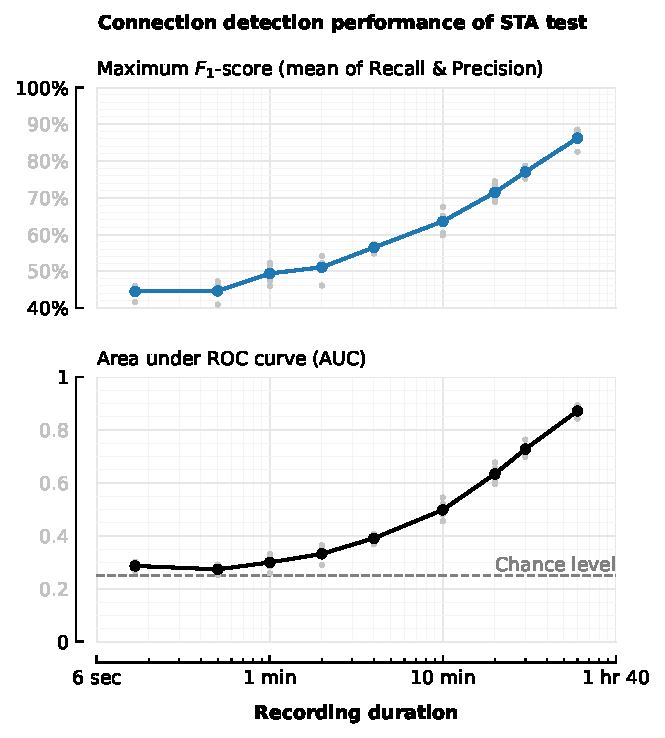
\includegraphics{STA_perf_diff_rec_duration}
    \end{sidecaption}
\end{figure}


\FloatBarrier
\section{Computational cost of STA test}

\begin{figure}
    \begin{sidecaption}
        {\textbf{Test time scales linearly with voltage signal duration}.\\
        Simulation timestep ('sample time') of 0.1 ms. STA length of 20 ms; i.e. 200 samples.
        The chosen inputs to test (300 high firing trains) have a median firing rate of 16 Hz. I.e. at a simulation duration of 10 seconds, there are about 160 presynaptic spikes per tested connection. There are 101 times that many STAs to calculate per connection: once for the real spiketrain, and a 100 times for shuffles of it. For a 10 second simulation, there are thus about 16k STAs to calculate per connection.
        For 10 minutes: 967k STAs. For 1 hour: 5.8M STAs.\\
        Black dots are the means over five simulations per duration. Compute times for individual simulations are plotted with gray dots; but the variation is so small that these gray dots are hidden behind the black means. Gray dashed line is the $y = x$ identity.  Source: \nburl{2023-09-20__STA_conntest_for_diff_recording_quality_n_durations}.}
        [fig:STA_compute_time]
        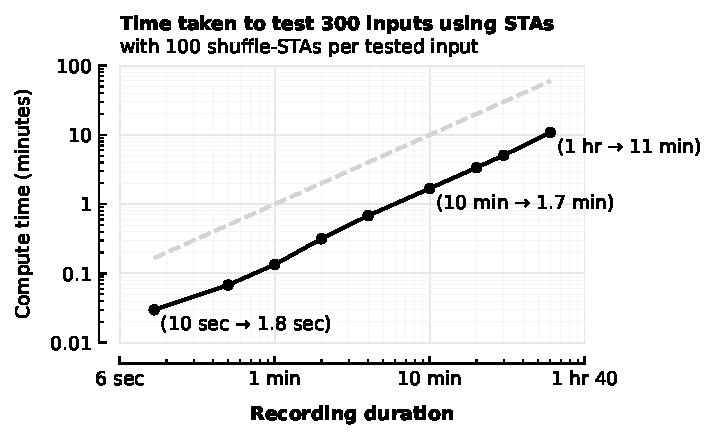
\includegraphics{STA_compute_time}
    \end{sidecaption}
    % This cap too long. some info → broodtext
\end{figure}
